\documentclass[a4paper, titlepage, 11pt]{article}

\usepackage[swedish]{babel}
\usepackage[T1]{fontenc}
\usepackage{lmodern}
\usepackage[utf8]{inputenc}
\usepackage{mathtools}
\usepackage{graphicx}
\usepackage{float}
\usepackage[table,xcdraw]{xcolor} % för snyggare tabeller

\setlength{\parindent}{0em}
\setlength{\parskip}{1em}

\title{Rapport för projekt: Kretsen}
\author{Grupp: Kretsen 6 \\ \\
Viola Söderlund \\ XXXXXX-XXXX \\ violaso@kth.se \\ \\
Jakob Carlsson \\ XXXXXX-XXXX \\ jakobcar@kth.se}

\begin{document}

\maketitle

\section{Frekvens och svängningstid med konstant L}
Vi vet att I(t) ska vara periodisk, vilket betyder att den kan skrivas på formen
$$I(t) = A*\sin(B*t + D)$$

Detta ger oss
\begin{gather*}
    I(t) = A*\sin(B*t + D) \\
    \implies I'(t) = A*B*\cos(B*t + D) \\
    \implies I''(t) = -A*B^2*\sin(B*t + D)
\end{gather*}

och givet relationerna (om L är konstant)
\begin{gather}
    U = L*I' \implies U' = L*I'' \\ % ej ekvivalens
    I = -C*U' \iff I = -(L*C*I'') \iff \frac{1}{-C*L} * I = I''
\end{gather}

får vi att
\begin{gather*}
    \frac{1}{-C*L} * A*sin(B*t + D) = -A*B^2*sin(B*t + D) \\
    \iff -B^2 = -\frac{1}{C*L} \\
    \iff B = \sqrt{\frac{1}{C*L}}
\end{gather*}

Med $L = L_0 = 0.7$ och det givna värdet $C = 0.5*10^{-6}$ får man:

\begin{gather*}
    p = \frac{2\pi}{\sqrt{\frac{1}{C*L}}} \approx 0,0037 \\
    fq = \frac{1}{p} \approx 269.0210
\end{gather*}

Dessa värden är exakta (till maskinnogrannheten) eftersom de räknades ut analytiskt och inte numeriskt. Detta hjälper oss att välja en rimlig intervallbredd senare, eftersom den ju bör vara (mycket) mindre än perioden p.


\section{Plotter av strömkurvorna vid olika U\textsubscript{0}}
Enligt projektbeskrivningen använder vi Runge-Kutta 4 för att räkna ut stömkurvorna givet tre olika värden på U\textsubscript{0}, nämligen 220 V, 1500 V och 2300 V.

Med hjälp av resultatet i förra sektionen kan vi välja en rimlig steglängd h för metoden, t.ex.
$h = 1*10^{-6}$.


Här stötte vi på ett problem. Relationerna givna i instruktionerna
\begin{gather*}
    U(t) = L(I) * I'(t) \\
    I(t) = -C * U'(t)
\end{gather*}
divergerar.

Om vi byter plats på -C och L, så får vi relationer som ger resultat som passar med hur de beskrivs i instruktionerna. På grund av detta använder vi dessa relationer istället. 
\begin{gather*}
    U(t) = -C * I'(t) \\
    I(t) = L(I) * U'(t)
\end{gather*}

Se sektion 3 för vidare diskussion om detta.

Vi definierar $y' = F(t, y)$ enligt:
\begin{gather*}
 y(t) = [U(t); I(t)] = [-C * I'(t); L(I) * U'(t)] \\
 \implies y'(t) = [I'(t); U'(t)] = [U(t)/(-C); I(t)/L(I)] =: F(t, y)
\end{gather*}

Vilket ger strömkurvorna:

\begin{figure}[H]
  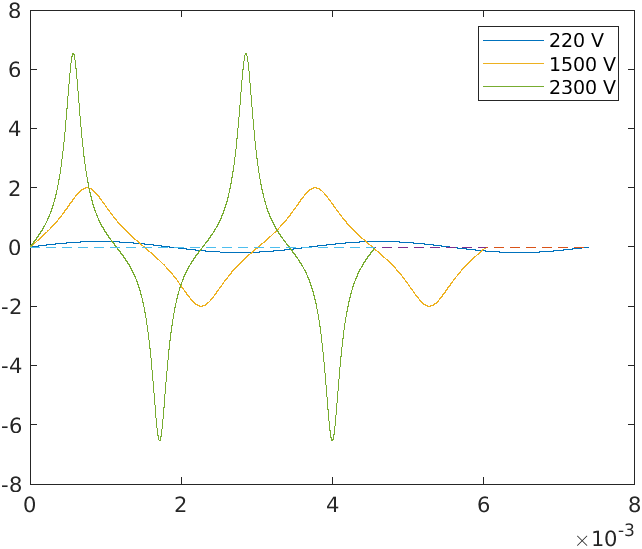
\includegraphics[width=\linewidth]{currents3.png}
  \caption{Två perioder av strömkurvorna vid några olika U\textsubscript{0}}
\end{figure}

Startvärdena var alltså I\textsubscript{0} = 0 och tre olika U\textsubscript{0} enligt figuren.


\section{Energin i spolen och kondensatorn}
Den totala energin $E(t)$ i systemet ska vara konstant. Detta beror på att det är modellerat som ett slutet system. Om inte energin då är konstant skulle vi ju bryta mot termodynamikens första huvudsats.

Utöver (1) och (2) från tidigare har vi också:
\begin{gather}
    L(I(t)) = L_0 * \frac{I_0^2}{I_0^2 + I(t)^2}
\end{gather}

Vi deriverar
$$E(t) = \frac{1}{2}CU(t)^2 + \frac{1}{2}L_0*I_0^2*\ln(I_0^2 + I(t)^2)$$
och visar med hjälp av sambanden att $E'(t) = 0 \implies E(t) =$ konstant.
\begin{gather*}
    E'(t) \\ = \\
    C*U(t)*U'(t) \\
    + \\
    \frac{1}{2}*L_0*I_0^2 * \frac{I(t)I'(t)}{I_0^2 + I(t)^2} \\
    = \\
    C*U(t)*U'(t) \\
    + \\
    \frac{L_0*I_0^2}{I_0^2 + I(t)^2}*I(t)I'(t) \\
    = \\
    C*U(t)*U'(t) + L(I(t)) * I(t)I'(t) \\
    = \\
    -I(t)U(t) + U(t)I(t) = 0
\end{gather*}

Vi simulerar även E(t) över ett stort antal perioder ($p = 40$). Vi gör detta genom att köra Runge-Kutta som tidigare med dels samma steglängd $h_1 = 10^{-6}$, och dels med en större steglängd $h_2 = 10^{-4}$. Sedan applicerar vi bara formeln för E vektorvis över hela resultatet.

\begin{figure}[H]
  \includegraphics[width=\linewidth]{E-smallH.png}
  \caption{E(t) över 40 perioder av I(t) med några olika U\textsubscript{0}, och med h = 10\textsuperscript{-6}}
\end{figure}

\begin{figure}[H]
  \includegraphics[width=\linewidth]{E-bigH.png}
  \caption{E(t) över 40 perioder av I(t) med några olika U\textsubscript{0}, och med h = 10\textsuperscript{-4}}
\end{figure}

Vi ser här att det är viktigt att ha en tillräckligt liten steglängd för att resultatet ska bli korrekt.

Något intressant här är att när vi visar analytiskt att E(t) är konstant använder vi relationerna som gavs i instruktionerna. När vi simulerar och visar på det sättet använder vi de modifierade relationerna som diskuterades i sektion 2.

\section{Strömmens toppvärde och periodtid}
Här används styckvis linjär interpolation.

JAG FÖRSTÅR ÄRLIGT TALAT INTE HUR FUNKTIONEN FUNGERAR, SÅ JAG KAN INTE SKRIVA NÅGOT RIMLIGT HÄR ANNAT ÄN RESULTATEN.

\begin{table}[H]
\caption{Strömmens maxvärde I\textsubscript{max} och periodlängd T beroende på spänningen U\textsubscript{0}. Felet ligger alltid i sista decimalen, som kan vara fel på grund av avrundning.}
\begin{center}
\begin{tabular}{l|lll}
\hline
\textbf{U\textsubscript{0}}   & 220    & 1500   & 2300   \\ \hline
\textbf{I\textsubscript{max}} & 0.187553 & 1.997132 & 6.5386 \\
\textbf{T}    & 0.03701  & 0.003019 & 0.002285
\end{tabular}
\end{center}
\end{table}

\begin{table}[H]
\caption{Rådata för tillförlitlighetsbedömning, där $h=10^{-6}$}
\begin{center}
\begin{tabular}{l|ll}
\hline
{\color[HTML]{000000} \textbf{U\textsubscript{0}, h}}     & {\color[HTML]{000000} \textbf{I\textsubscript{max}}}   & {\color[HTML]{000000} \textbf{T}}        \\ \hline
{\color[HTML]{000000} \textbf{220, h}}    & {\color[HTML]{000000} 0.187552548575790} & {\color[HTML]{000000} 0.003700568248926} \\
{\color[HTML]{000000} \textbf{220, h/2}}  & {\color[HTML]{000000} 0.187552558040406} & {\color[HTML]{000000} 0.003701068248639} \\
{\color[HTML]{000000} \textbf{220, h/4}}  & {\color[HTML]{000000} 0.187552570642913} & {\color[HTML]{000000} 0.003701068248619} \\ \hline
{\color[HTML]{000000} \textbf{1500, h}}   & {\color[HTML]{000000} 1.997132052304110} & {\color[HTML]{000000} 0.003018680878398} \\
{\color[HTML]{000000} \textbf{1500, h/2}} & {\color[HTML]{000000} 1.997132052303030} & {\color[HTML]{000000} 0.003019180878903} \\
{\color[HTML]{000000} \textbf{1500, h/4}} & {\color[HTML]{000000} 1.997132298244580} & {\color[HTML]{000000} 0.003019180878994} \\ \hline
{\color[HTML]{000000} \textbf{2300, h}}   & {\color[HTML]{000000} 6.538558656458210} & {\color[HTML]{000000} 0.002284745598040} \\
{\color[HTML]{000000} \textbf{2300, h/2}} & {\color[HTML]{000000} 6.538608843205730} & {\color[HTML]{000000} 0.002285245599219} \\
{\color[HTML]{000000} \textbf{2300, h/4}} & {\color[HTML]{000000} 6.538609292790240} & {\color[HTML]{000000} 0.002285245599511}
\end{tabular}
\end{center}
\end{table}


\section{Hitta spänningen U\textsubscript{0}\textsuperscript{*} för frekvensen 400 Hz}
Här använder vi sekantmetoden för att lösa ekvationen VAD ÄR EKVATIONEN??

Startgissningarna kommer från förra sektionen. Eftersom vi söker en frekvens på 400 Hz, dvs. $T = \frac{1}{400} = 0.0025$, och vi hade
\begin{gather*}
    U_0 = 2300 \implies T = 0.0023 < 0.0025 \\
    U_0 = 1500 \implies T = 0.0030 > 0.0025
\end{gather*}
så är dessa två värden på U\textsubscript{0} rimliga att använda som startgissningar.

Detta ger oss värdet $U_0^* = 2069$ vilket ger ett maxvärde på strömmen $I_{max}^* = 4.5031$. Alla siffror i dessa tal är korrekta. Mer specifikt är felet på $U_0^*$ i storleksordningen $10^{-3}$ och felet på $I_{max}^*$ är i storleksordningen $10^{-6}$.

\begin{table}[H]
\caption{Rådata för tillförlitlighetsbedömning, olika steglängder och toleranser. $h = 10^{-6}$, eps $= 2.220446049250313*10^{-16}$ }
\begin{center}
\begin{tabular}{l|ll}
\hline
{\color[HTML]{000000} \textbf{h, tol}}     & {\color[HTML]{000000} \textbf{U\textsuperscript{*}\textsubscript{0}}}     & {\color[HTML]{000000} \textbf{I\textsuperscript{*}\textsubscript{max}}}  \\ \hline
{\color[HTML]{000000} \textbf{h, 1e-10}}   & {\color[HTML]{000000} 2068.99484901206} & {\color[HTML]{000000} 4.50310419770553} \\
{\color[HTML]{000000} \textbf{h, 1e-15}}   & {\color[HTML]{000000} 2068.99500936829} & {\color[HTML]{000000} 4.50310531749166} \\
{\color[HTML]{000000} \textbf{h, eps}}     & {\color[HTML]{000000} 2068.99500936911} & {\color[HTML]{000000} 4.50310531749737} \\ \hline
{\color[HTML]{000000} \textbf{h/2, 1e-10}} & {\color[HTML]{000000} 2068.99481404489} & {\color[HTML]{000000} 4.50310395344584} \\
{\color[HTML]{000000} \textbf{h/2, 1e-15}} & {\color[HTML]{000000} 2068.99500936242} & {\color[HTML]{000000} 4.50310531737086} \\
{\color[HTML]{000000} \textbf{h/2, eps}}   & {\color[HTML]{000000} 2068.99500936338} & {\color[HTML]{000000} 4.50310531737757} \\ \hline
{\color[HTML]{000000} \textbf{h/4, 1e-10}} & {\color[HTML]{000000} 2068.99485072491} & {\color[HTML]{000000} 4.50310420958168} \\
{\color[HTML]{000000} \textbf{h/4, 1e-15}} & {\color[HTML]{000000} 2068.99500936160} & {\color[HTML]{000000} 4.50310531736015} \\
{\color[HTML]{000000} \textbf{h/4, eps}}   & {\color[HTML]{000000} 2068.99500936317} & {\color[HTML]{000000} 4.50310531737108}
\end{tabular}
\end{center}
\end{table}


\section{Osäkerhet i modellen}
Om man varierar L\textsubscript{0} och C vardera med $\pm5\%$ får man att största felet på $U_0^*$ är ungefär $140$ och det största felet på $I_{max}^*$ är ungefär $1.01$. Detta är betydligt större än de numeriska felen från förra sektionen.

\begin{table}[H]
\caption{Rådata för felen i $U_0^*$ och $I_{max}^*$.}
\begin{center}
\begin{tabular}{l|ll}
\hline
\textbf{indatastörning, $5\% * [L_0, C]$} & \textbf{abs{[}felet i U*\textsubscript{0}{]}}         & \textbf{abs{[}felet i I*\textsubscript{max}{]}}     \\ \hline
\textbf{-1, 0}          & {\color[HTML]{000000} 119.7911953379} & {\color[HTML]{000000} 0.4529453012} \\
\textbf{1, 0}           & {\color[HTML]{000000} 116.9956676344} & {\color[HTML]{000000} 0.4777440246} \\
\textbf{0, -1}          & {\color[HTML]{000000} 17.2015209153}  & {\color[HTML]{000000} 0.4529453012} \\
\textbf{0, 1}           & {\color[HTML]{000000} 12.9008734915}  & {\color[HTML]{000000} 0.4777440246} \\
\textbf{-1, -1}         & {\color[HTML]{000000} 140.1589962046} & {\color[HTML]{000000} 0.8617237602} \\
\textbf{-1, 1}          & {\color[HTML]{000000} 104.1614611061} & {\color[HTML]{000000} 0.0232231367} \\
\textbf{1, -1}          & {\color[HTML]{000000} 102.6631229215} & {\color[HTML]{000000} 0.0232231367} \\
\textbf{1, 1}           & {\color[HTML]{000000} 127.4086699916} & {\color[HTML]{000000} 1.007785437} 
\end{tabular}
\end{center}
\end{table}


\section{Egen arbetsinsats}



\end{document}
